%%%%%%%%%%%%%%%%%%%%%%%%%%%%%%%%%%%%

\section{ケーススタディ：性差別}

%%%%%%%%%%%%%%%%%%%%%%%%%%%%%%%%%%%%

\subsection{研究の説明とデータ}

%%%%%%%%%%%%%%%%%%%%%%%%%%%%%%%%%%%%

\begin{frame}[shrink=15]
\frametitle{性差別}

\begin{itemize}

\item 1972年、性差別研究の一環として、48名の男性銀行管理職がそれぞれ同じ人事ファイルを渡され、
その人物を「通常業務」と説明された支店長職に昇進させるべきかどうかを判断するよう求められた。

\item ファイルは同一だったが、管理職の半数は男性を示すファイルを、残り半数は女性を示すファイルを受け取った。

\item どの管理職が「男性」応募書類を受け取り、どの管理職が「女性」応募書類を受け取るかはランダムに決定された。

\item 審査された48件のファイルのうち、35件が昇進を推薦された。

\item この研究は女性が不当に差別されているかどうかを検証している。

\end{itemize}

\dq{これは観察研究か実験か？} \soln{実験}

\ct{B.Rosen and T. Jerdee (1974), ``Influence of sex role stereotypes on personnel decisions", J.Applied Psychology, 59:9-14.}

\end{frame}


%%%%%%%%%%%%%%%%%%%%%%%%%%%%%%%%%%%%

\begin{frame}
\frametitle{データ}

\dq{一見して、昇進と性別の間に関係があるように見えるか？}

\begin{center}
\begin{tabular}{ll  cc c}
        &               & \multicolumn{2}{c}{\textit{昇進}} \\
\cline{3-4}
                        &           & 昇進あり  & 昇進なし  & 合計  \\
\cline{2-5}
\multirow{2}{*}{\textit{性別}}  &男性    & 21        & 3     & 24    \\
                        &女性        & 14        & 10    & 24 \\
\cline{2-5}
                        &合計        & 35        & 13    & 48 \\
\end{tabular}
\end{center}

\textbf{昇進した男性の割合：$21 / 24 = 0.875$} \\
\textbf{昇進した女性の割合：$14 / 24 = 0.583$}

\end{frame}

%%%%%%%%%%%%%%%%%%%%%%%%%%%%%%%%%%%%

\begin{frame}[shrink=25]
\frametitle{練習問題}

\pq{昇進推薦された男性と女性ファイルの割合に約30\%（正確には29.2\%）の差があることが分かった。この情報に基づいて、以下のうち正しいものはどれか？}

\begin{enumerate}[(a)]

\item 実験を繰り返せば、必ずより多くの女性ファイルが昇進推薦される。今回はまぐれだった。

\item 昇進は性別に依存しており、男性の方が昇進しやすく、昇進決定において女性への性差別がある。\only<2->{\red{かもしれない}}

\item 昇進した男性と女性ファイルの割合の差は偶然によるものであり、昇進決定における女性への性差別の証拠ではない。\only<2->{\red{かもしれない}}

\item 女性は男性より能力が低く、そのためより少ない女性が昇進する。

\end{enumerate}

\end{frame}

%%%%%%%%%%%%%%%%%%%%%%%%%%%%%%%%%%%%

\subsection{競合する主張}

%%%%%%%%%%%%%%%%%%%%%%%%%%%%%%%%%%%%%

\begin{frame}
\frametitle{2つの競合する主張}

\begin{enumerate}

\item 「何も起きていない。」\\
昇進と性別は\hl{独立}であり、性差別はなく、割合の差は単に偶然による。$\rightarrow$ \hl{帰無仮説}

\item 「何かが起きている。」\\
昇進と性別は\hl{従属}であり、性差別があり、割合の差は偶然ではない。$\rightarrow$ \hl{対立仮説}

\end{enumerate}

\end{frame}

%%%%%%%%%%%%%%%%%%%%%%%%%%%%%%%%%%%%

\begin{frame}[shrink=25]
\frametitle{仮説検定としての裁判}

\twocol{0.5}{0.5}
{
\begin{itemize}

\item 仮説検定は裁判によく似ている。

\item $H_0$：被告は無実 \\
$H_A$：被告は有罪

\item 次に証拠を提示する――データを収集する。

\end{itemize}
}
{
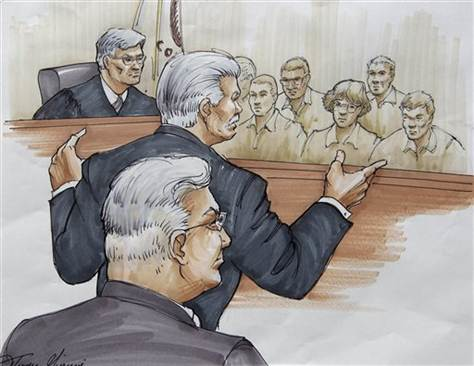
\includegraphics[width=0.85\textwidth]{2-3_gender_discrimination/figures/trial}
}

\begin{itemize}

\item 次に証拠を判断する――「帰無仮説が真であった場合、これらのデータが偶然に起こりうるか？」
\begin{itemize}
\item それが起こる可能性が非常に低い場合、証拠は帰無仮説について合理的な疑いを超える疑念を生じさせる。
\end{itemize}

\item 最終的には決断を下さなければならない。どれほど低い確率を「起こりにくい」と言うのか？

\end{itemize}

\ct{Image from \webURL{http://www.nwherald.com/_internal/cimg!0/oo1il4sf8zzaqbboq25oevvbg99wpot}.}

\end{frame}

%%%%%%%%%%%%%%%%%%%%%%%%%%%%%%%%%%%%%

\begin{frame}[shrink=15]
\frametitle{仮説検定としての裁判（続き）}

\begin{itemize}

\item 証拠が無実の仮定を棄却するのに十分でない場合、陪審員は「無罪」の評決を下す。
\begin{itemize}
\item 陪審員は被告が無実とは言わず、有罪にするための証拠が十分でないと言うだけである。
\item 被告は実際に無実かもしれないが、陪審員には確かめる方法がない。
\end{itemize}

\item 統計的には、\textbf{帰無仮説を棄却できない}と言う。
\begin{itemize}
\item 帰無仮説が真かどうかを単純に知ることができないため、帰無仮説が真であるとは決して宣言しない。
\item そのため、「帰無仮説を採択する」とは決して言わない。
\end{itemize}

\end{itemize}

\end{frame}

%%%%%%%%%%%%%%%%%%%%%%%%%%%%%%%%%%%%%

\begin{frame}
\frametitle{仮説検定としての裁判（続き）}

\begin{itemize}

\item 裁判では、証明責任は検察側にある。

\item 仮説検定では、証明責任は異常な主張の側にある。

\item 帰無仮説は通常の状態（現状）であるため、異常とみなされるのは対立仮説であり、その証拠を集める必要がある。

\end{itemize}

\end{frame}

%%%%%%%%%%%%%%%%%%%%%%%%%%%%%%%%%%%%%

\begin{frame}
\frametitle{まとめ：仮説検定の枠組み}

\begin{itemize}
\item 現状を表す\hl{帰無仮説（$H_0$）}から始める。
\item また、研究の問い（何を検証するか）を表す\hl{対立仮説（$H_A$）}もある。
\item 帰無仮説が真であるという仮定のもとで、シミュレーション（今回）または理論的方法（後の講義）によって仮説検定を行う。
\item 検定結果が対立仮説を支持する説得力のある証拠を示さない場合は帰無仮説を維持し、示す場合は帰無仮説を棄却して対立仮説を採択する。
\end{itemize}

\end{frame}

%%%%%%%%%%%%%%%%%%%%%%%%%%%%%%%%%%%%

\subsection{シミュレーションによる検証}

%%%%%%%%%%%%%%%%%%%%%%%%%%%%%%%%%%%%%

\begin{frame}
\frametitle{実験のシミュレーション…}

…独立性の仮定のもと、つまり偶然に委ねる。\\

\vspace{0.5cm}

\hl{偶然モデル}に基づくシミュレーションの結果がデータに似ている場合、男女間の昇進ファイルの割合の差は単に\hl{偶然によるもの}と判断できる（昇進と性別は独立）。\\

\vspace{0.5cm}

偶然モデルに基づくシミュレーションの結果がデータに似ていない場合、男女間の昇進ファイルの割合の差は偶然ではなく、\hl{性別の実際の影響}によるものと判断できる（昇進と性別は従属）。

\end{frame}

%%%%%%%%%%%%%%%%%%%%%%%%%%%%%%%%%%%%

\begin{frame}[shrink=10]
\frametitle{応用活動：実験のシミュレーション}

\app{
トランプを使ってこの実験をシミュレートせよ。

\begin{enumerate}
\item 絵札を「昇進なし」、数札を「昇進あり」とする。エースは絵札として扱う。
\begin{itemize}
\item ジョーカーを取り除く。
\item エース3枚を取り除く $\rightarrow$ デッキに絵札がちょうど13枚残る（絵札：A, K, Q, J）。
\item 数札1枚を取り除く $\rightarrow$ デッキに数札がちょうど35枚残る（数札：2〜10）。
\end{itemize}
\item カードをシャッフルし、男性と女性を表す24枚ずつの2グループに配る。
\item 各グループで昇進推薦された（数札）ファイルの数を数えて記録する。

\item 各グループの昇進推薦ファイルの割合を計算し、差（男性 $-$ 女性）を求めて記録する。

\item ステップ2〜4を多数回繰り返す。

\end{enumerate}
}

\end{frame}

%%%%%%%%%%%%%%%%%%%%%%%%%%%%%%%%%%%%

\begin{frame}
\frametitle{ステップ1}

\begin{center}
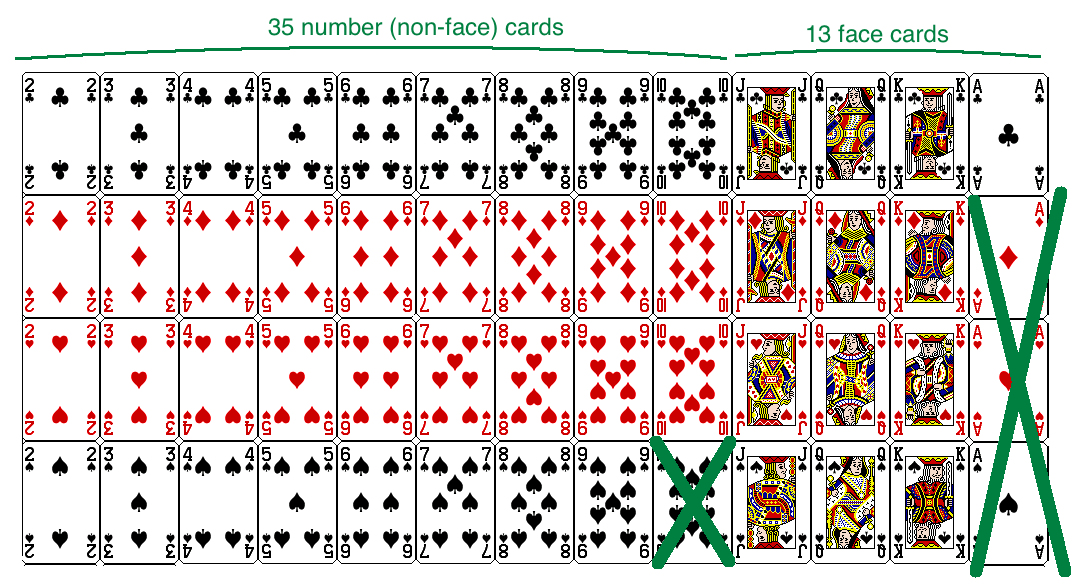
\includegraphics[width=\textwidth]{2-3_gender_discrimination/figures/step1}
\end{center}

\end{frame}


%%%%%%%%%%%%%%%%%%%%%%%%%%%%%%%%%%%%

\begin{frame}
\frametitle{ステップ2〜4}

\begin{center}
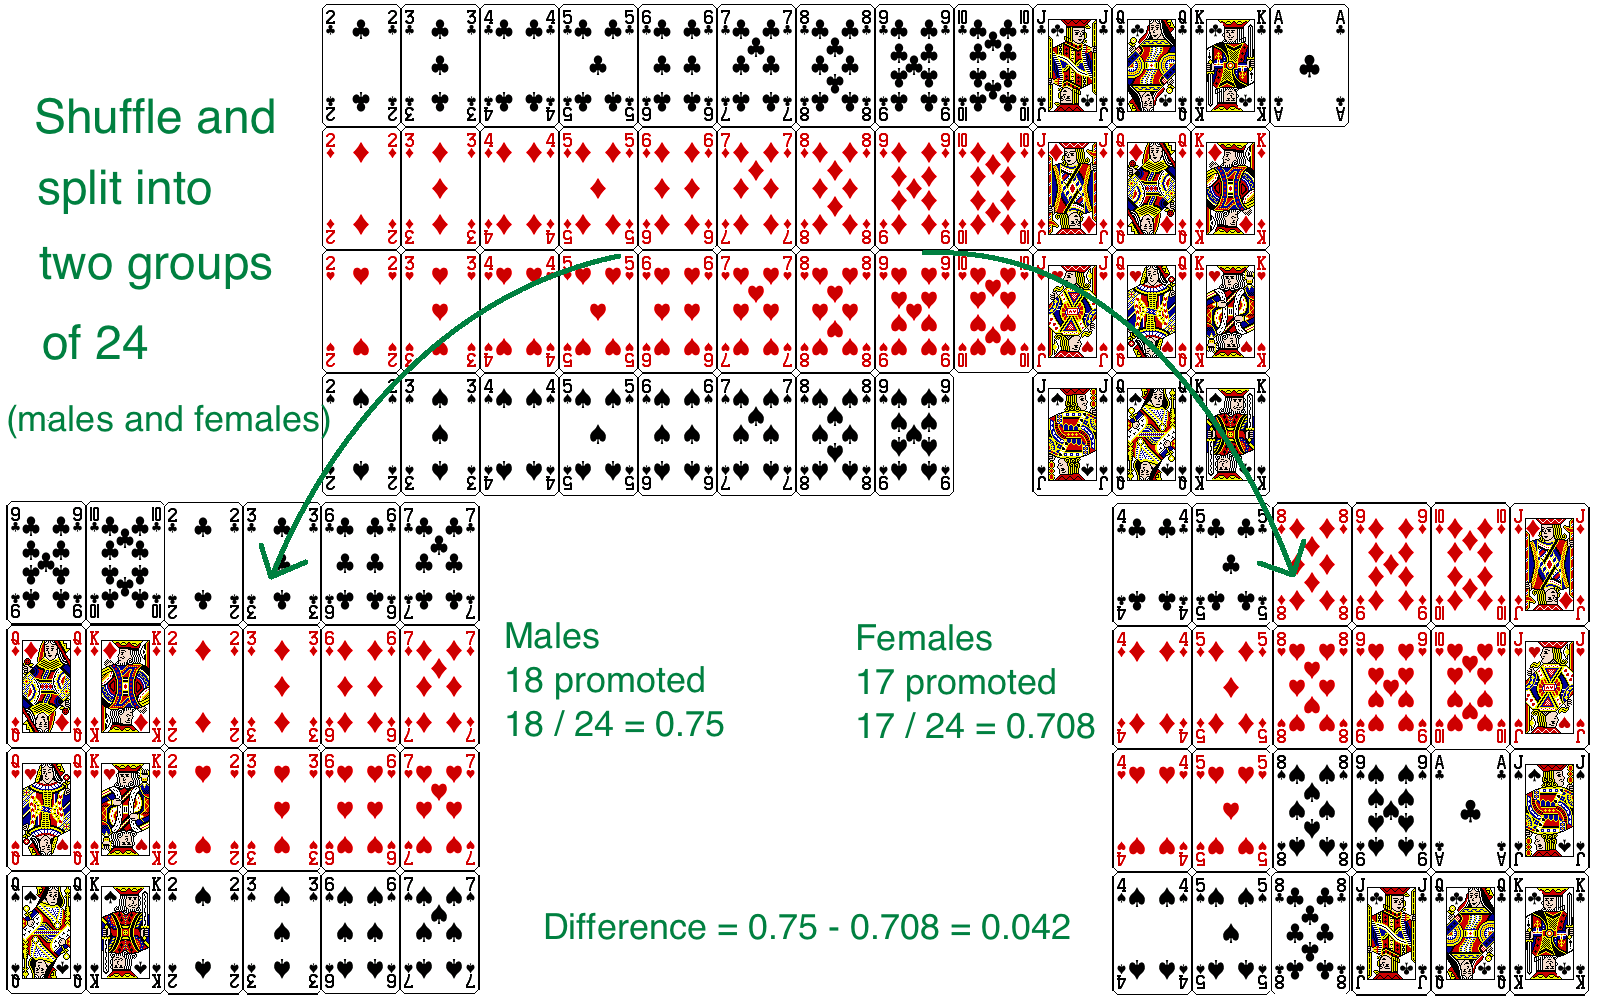
\includegraphics[width=\textwidth]{2-3_gender_discrimination/figures/step2}
\end{center}

\end{frame}


%%%%%%%%%%%%%%%%%%%%%%%%%%%%%%%%%%%%

\subsection{独立性の確認}

%%%%%%%%%%%%%%%%%%%%%%%%%%%%%%%%%%%%

\begin{frame}
\frametitle{練習問題}

\pq{今実施したシミュレーションの結果は、女性への性差別（つまり性別と昇進決定の従属関係）の説得力のある証拠を提供するか？}

\begin{enumerate}[(a)]
\item いいえ。データは対立仮説を支持する説得力のある証拠を提供しないため、性別と昇進決定の独立性という帰無仮説を棄却できない。2つの割合の差は偶然によるものだった。
\solnMult{はい。データは昇進決定における女性への性差別という対立仮説を支持する説得力のある証拠を提供する。2つの割合の差は性別の実際の影響によるものだった。}
\end{enumerate}

\end{frame}

%%%%%%%%%%%%%%%%%%%%%%%%%%%%%%%%%%%%

\begin{frame}
\frametitle{ソフトウェアによるシミュレーション}

前述の方法でシミュレーションを実行するのは面倒で時間がかかる。実際にはソフトウェアを使ってシミュレーションを生成する。下のドットプロットは100回のシミュレーションに基づく昇進率の差のシミュレーション分布を示す。

\begin{center}
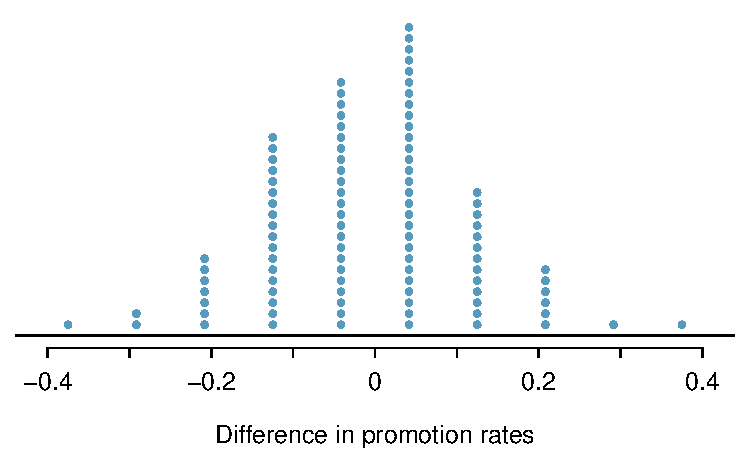
\includegraphics[width=0.7\textwidth]{2-3_gender_discrimination/figures/discRandDotPlot/discRandDotPlot}
\end{center}

\end{frame}

%%%%%%%%%%%%%%%%%%%%%%%%%%%%%%%%%%%%%
